%! TEX root = analisis_iklim_temu8.tex
% the main TeX file which is intended to compile, :VimtexReload after adjustment
% :h vimtex-tex-root
\documentclass[../main.tex]{subfiles}
% \includeonlyframes{current}
% \setbeameroption{hide notes} % Only slides
% \setbeameroption{show only notes} % Only notes
% \setbeameroption{show notes on second screen=right} % Both

\begin{document}


\begin{frame}[mytitle=standard,c,mycolor=digiPH_gray,light]
	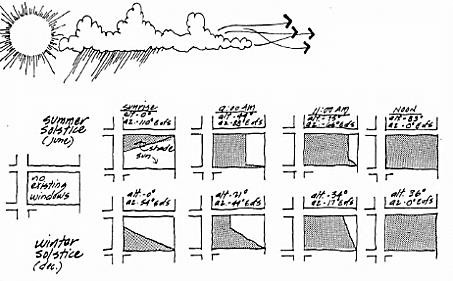
\includegraphics[width=.86\textwidth]{../figures/iklim_1}
\end{frame}
\begin{frame}[mytitle=standard,c,mycolor=digiPH_gray,light]
	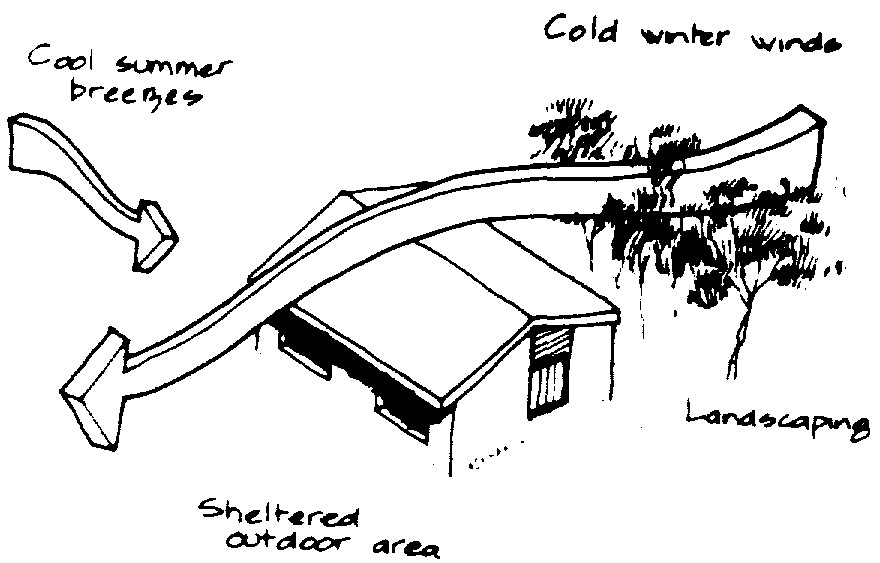
\includegraphics[width=.86\textwidth]{../figures/iklim_2}
\end{frame}

\begin{frame}[mytitle=standard,c,mycolor=digiPH_gray,light]
	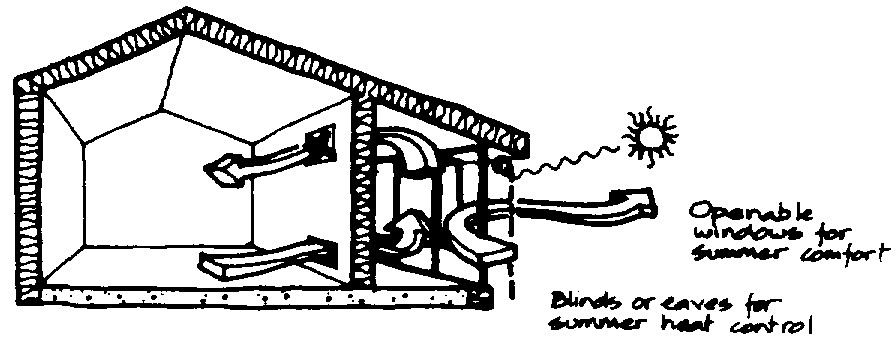
\includegraphics[width=.86\textwidth]{../figures/iklim_3}
\end{frame}

\begin{frame}[mytitle=standard,c,mycolor=digiPH_gray,light]
	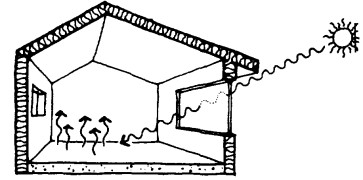
\includegraphics[width=.86\textwidth]{../figures/iklim_4}
\end{frame}

\bgdarkimg{iklim_5}
\bgdarkimg{iklim_6}
\bgdarkimg{iklim_7}

\bgdarkimg{iklim_cth}
\bgdarkimg{iklim_2_cth}
\bgdarkimg{iklim_3_cth}

\end{document}
